%
% ---------------------------------------------------------------
% Copyright (C) 2012-2018 Gang Li
% ---------------------------------------------------------------
%
% This work is the default powerdot-tuliplab style test file and may be
% distributed and/or modified under the conditions of the LaTeX Project Public
% License, either version 1.3 of this license or (at your option) any later
% version. The latest version of this license is in
% http://www.latex-project.org/lppl.txt and version 1.3 or later is part of all
% distributions of LaTeX version 2003/12/01 or later.
%
% This work has the LPPL maintenance status "maintained".
%
% This Current Maintainer of this work is Gang Li.
%
%

\documentclass[
 size=14pt,
 paper=smartboard,  %a4paper, smartboard, screen
 mode=present, 		%present, handout, print
 display=slides, 	% slidesnotes, notes, slides
 style=tuliplab,  	% TULIP Lab style
 pauseslide,
 fleqn,leqno]{powerdot}


\usepackage{cancel}
\usepackage{caption}
\usepackage{stackengine}
\usepackage{smartdiagram}
\usepackage{attrib}
\usepackage{amssymb}
\usepackage{amsmath} 
\usepackage{amsthm} 
\usepackage{mathtools}
\usepackage{rotating}
\usepackage{graphicx}
\usepackage{boxedminipage}
\usepackage{rotate}
\usepackage{calc}
\usepackage[absolute]{textpos}
\usepackage{psfrag,overpic}
\usepackage{fouriernc}
\usepackage{pstricks,pst-3d,pst-grad,pstricks-add,pst-text,pst-node,pst-tree}
\usepackage{moreverb,epsfig,subfigure}
\usepackage{color}
\usepackage{booktabs}
\usepackage{etex}
\usepackage{breqn}
\usepackage{multirow}
\usepackage{natbib}
\usepackage{bibentry}
\usepackage{gitinfo2}
\usepackage{siunitx}
\usepackage{nicefrac}
%\usepackage{geometry}
%\geometry{verbose,letterpaper}
\usepackage{media9}
\usepackage{animate}
%\usepackage{movie15}
\usepackage{auto-pst-pdf}

\usepackage{breakurl}
\usepackage{fontawesome}
\usepackage{xcolor}
\usepackage{multicol}



\usepackage{verbatim}
\usepackage[utf8]{inputenc}
\usepackage{dtk-logos}
\usepackage{tikz}
\usepackage{adigraph}
%\usepackage{tkz-graph}
\usepackage{hyperref}
%\usepackage{ulem}
\usepackage{pgfplots}
\usepackage{verbatim}
\usepackage{fontawesome}


\usepackage{todonotes}
% \usepackage{pst-rel-points}
\usepackage{animate}
\usepackage{fontawesome}

\usepackage{listings}
\lstset{frameround=fttt,
frame=trBL,
stringstyle=\ttfamily,
backgroundcolor=\color{yellow!20},
basicstyle=\footnotesize\ttfamily}
\lstnewenvironment{code}{
\lstset{frame=single,escapeinside=`',
backgroundcolor=\color{yellow!20},
basicstyle=\footnotesize\ttfamily}
}{}


\usepackage{hyperref}
\hypersetup{ % TODO: PDF meta Data
  pdftitle={Presentation Title},
  pdfauthor={Gang Li},
  pdfpagemode={FullScreen},
  pdfborder={0 0 0}
}


% \usepackage{auto-pst-pdf}
% package to show source code

\definecolor{LightGray}{rgb}{0.9,0.9,0.9}
\newlength{\pixel}\setlength\pixel{0.000714285714\slidewidth}
\setlength{\TPHorizModule}{\slidewidth}
\setlength{\TPVertModule}{\slideheight}
\newcommand\highlight[1]{\fbox{#1}}
\newcommand\icite[1]{{\footnotesize [#1]}}

\newcommand\twotonebox[2]{\fcolorbox{pdcolor2}{pdcolor2}
{#1\vphantom{#2}}\fcolorbox{pdcolor2}{white}{#2\vphantom{#1}}}
\newcommand\twotoneboxo[2]{\fcolorbox{pdcolor2}{pdcolor2}
{#1}\fcolorbox{pdcolor2}{white}{#2}}
\newcommand\vpspace[1]{\vphantom{\vspace{#1}}}
\newcommand\hpspace[1]{\hphantom{\hspace{#1}}}
\newcommand\COMMENT[1]{}

\newcommand\placepos[3]{\hbox to\z@{\kern#1
        \raisebox{-#2}[\z@][\z@]{#3}\hss}\ignorespaces}

\renewcommand{\baselinestretch}{1.2}


\newcommand{\draftnote}[3]{
	\todo[author=#2,color=#1!30,size=\footnotesize]{\textsf{#3}}	}
% TODO: add yourself here:
%
\newcommand{\gangli}[1]{\draftnote{blue}{GLi:}{#1}}
\newcommand{\shaoni}[1]{\draftnote{green}{sn:}{#1}}
\newcommand{\gliMarker}
	{\todo[author=GLi,size=\tiny,inline,color=blue!40]
	{Gang Li has worked up to here.}}
\newcommand{\snMarker}
	{\todo[author=Sn,size=\tiny,inline,color=green!40]
	{Shaoni has worked up to here.}}

%%%%%%%%%%%%%%%%%%%%%%%%%%%%%%%%%%%%%%%%%%%%%%%%%%%%%%%%%%%%%%%%%%%%%%%%
% title
% TODO: Customize to your Own Title, Name, Address
%
\title{Predict Future Sales}
\author{
Siyu Chen
\\
\\Xi'an Shiyou University

}
\date{\gitCommitterDate}


% Customize the setting of slides
\pdsetup{
% TODO: Customize the left footer, and right footer
rf=\href{http://www.tulip.org.au}{
Last Changed by: \textsc{\gitCommitterName}\ \gitVtagn-\gitAbbrevHash\ (\gitAuthorDate)
},
cf={Predict Future Sales},
}


\begin{document}

\maketitle

%\begin{slide}{Overview}
%\tableofcontents[content=sections]
%\end{slide}


%%==========================================================================================
%%
\begin{slide}[toc=,bm=]{Overview}
\tableofcontents[content=currentsection,type=1]
\end{slide}
%%
%%==========================================================================================


\section{Problem Definition}


%%==========================================================================================
%%
\begin{slide}{Analyze Data}
\begin{center}
\twotonebox{\rotatebox{90}{Files}}{\parbox{.86\textwidth}
{predict total sales for every product and store in the next month.
\begin{itemize}
\item sales_train.csv: Training set 2013 to October 2015.
\item test.csv: Test set forecast sales of these stores and products in November 2015.
\item items.csv: Additional information about the merchandise/product.
\item item_categories.csv: Additional information on the categories of goods.
\item shops.csv: Additional information about the store.
\end{itemize}
}}

\end{center}
\bigskip
\begin{center}
\end{center}
\bigskip

%%==========================================================================================
\begin{note}
First, I will introduce the problem definition.
In the real life,
a teacher may be interested in the characteristics that
make one student obvious different from others.
Or,
NBA sports coaches would prefer to
know the advantages and disadvantages of one player.
Here, the player can be regarded as a query object.

For example, team A has five players,
each player has four features.
The NBA sports coaches may want to know the features of
player $1$ that are different from others.

The above example can be seen as outlying aspects mining.
The main purpose of outlying aspects mining is to identify
the outstanding features of the query object.
\end{note}
%%==========================================================================================

\end{slide}
%%
%%==========================================================================================


%%==========================================================================================
%%
\begin{slide}[toc=,bm=]{File Field Description}
\begin{center}

\end{center}

\bigskip

\twocolumn[
\savevalue{lfrheight}=8cm,
\savevalue{lfrprop}={
linestyle=solid,framearc=.2,linewidth=1pt},
rfrheight=\usevalue{lfrheight},
rfrprop=\usevalue{lfrprop}
]{
  
\begin{itemize}
\item
\smallskip
\textcolor{orange}{shop_id} : unique identifier for a store.
\smallskip
\item
\smallskip
\textcolor{orange}{item_id} : A unique identifier for a product.
\smallskip
\item
\smallskip
\textcolor{orange}{item_category_id} : A unique identifier for a category.
\smallskip
\item
\smallskip
\textcolor{orange}{item_cnt_day} : Quantity of products sold.
\smallskip
\end{itemize}
}{

  \begin{itemize}
    \item
    \smallskip
    \textcolor{orange}{item_price} : The current price of the goods.
    \smallskip
    \item
    \smallskip
    \textcolor{orange}{date_block_num} : A consecutive month.
    \smallskip
    \item
    \smallskip
    \textcolor{orange}{item_name} : Product name.
    \smallskip
    \item
    \smallskip
    \textcolor{orange}{shop_name} : Shop name.
    \smallskip
    \item
    \smallskip
    \textcolor{orange}{item_category_name} : The name of the project category.
    \smallskip
    \end{itemize}
}

%%==========================================================================================
\begin{note}
Based on the above example,
I will compare the differences
between outlying aspects mining and outlier detection.

Outlying aspects mining aims to
explain the distinctive aspects of the query object.
The query object may or may not be an outlier.
In contrast,
Outlier detection aims to discover all possible
outlying objects in the dataset.
Without explaining how and why they are different.

Let's go back to the NBA example,
in that example,
the output of the outlying aspects mining may be
a combination of four features,
but the output of the outlier detection may be any of those five players.
\end{note}
%%==========================================================================================

\end{slide}
%%
\begin{slide}{Data Statistics}

  \begin{itemize}
  \item Statistic the data in the training set
  \end{itemize}
  
  \begin{table}
  \setlength{\abovecaptionskip}{0pt}
  \setlength{\belowcaptionskip}{10pt}
  \centering
  \caption{Statistic the data in the training set}
  
  \begin{tabular}{p{1.1cm}p{2.5cm}p{2.5cm}p{2.5cm}p{2.5cm}p{2.5cm}p{2.5cm}p{2.5cm}p{2.5cm}}
  \hline
    % after \\: \hline or \cline{col1-col2} \cline{col3-col4} ...
      & $datebknum$ & $shop\_id$ & $item\_id$ & $item\_price$ & $item cnt day$ & $item\_ctg\_id$\\
  \hline
    $count$   & 2935849.00 & 2935849.00  & 2935849.00  & 2935849.00  & 2935849.00  & 2935849.00 \\
    $mean$   & 14.57  & 33.00  & 10197.23  & 890.62  & 1.24 & 40.00 \\
    $std$   & 9.42  & 16.23 & 6324.30  & 1726.44 & 2.62 & 17.10 \\
    $min$   & 0.00  & 0.00  & 0.00  & -1.00  & -22.00 & 0.00 \\
    $25\%$   & 7.00    & 22.00  & 4476.00  & 249.00  & 1.00 & 28.00 \\
    $50\%$   & 14.00  & 31.00 & 9343.00 & 399.00  & 1.00  & 40.00 \\
    $75\%$   & 23.00  & 47.00  & 15684.00  & 999.00  & 1.00 & 55.00 \\
    $max$   & 33.00 & 59.00  & 22169.00 & 307980.00  & 2169.00 &83.00 \\
    
  \hline
  \end{tabular}
  \end{table}
  
  %%==========================================================================================
  \begin{note}
  Now,
  I am gonna use a synthetic dataset to verify our method.
  
  The dataset we used in our experiment contains $10$ groups,
  each group consists of $10$ members,
  and each member has $8$ features: $F_1$ to $F_8$.
  
  Table $5$ shows the original data of one group,
  and the bold features represent the ground truth,
  The ground truth include trivial outlying feature \{$F_1$\},
  and non-trivial outlying subspace \{$F_2$, $F_4$\}.
  \end{note}
  %%==========================================================================================
  
  \end{slide}
%%==========================================================================================
\section{Data Processing}

%%==========================================================================================
%%
\begin{slide}[toc=,bm=]{Three ways to process data}

  \begin{itemize}
  \item
  Once we get the data set, we need to process the data.
  
  \begin{itemize}
  \item
  Use only shop_id and item_id that appear in the test set.
  
  Data set size before: 2935849
  
  Data set size after: 1224439
  \item
  Use only data whose price is greater than 0.
  \item
  Drop the text features.
  \item
  Delete the unwanted columns, aggregate them monthly, and get a new data set.
  
  Get new features:Total monthly sales price item_price and Monthly gross sales item_cnt.
  \end{itemize}
  \end{itemize}
  
  %%==========================================================================================
  \begin{note}
  The second challenge is how to evaluate the outlying degree of
  the query group between different aspects.
  
  In that case,
  we need to design a scoring function to measure the outlying degree.
  But adopting an appropriate scoring function without dimension bias still remains a problem.
  \end{note}
  %%==========================================================================================
  
  \end{slide}
%%==========================================================================================


%%==========================================================================================
%%
\begin{slide}{Removing Outliers}
  \begin{itemize}
    \item
    Discard outliers
    
    \end{itemize}
    
    \begin{figure}
      \centering
      \selectcolormodel{rgb}
      %\missingfigure{Testing.}
      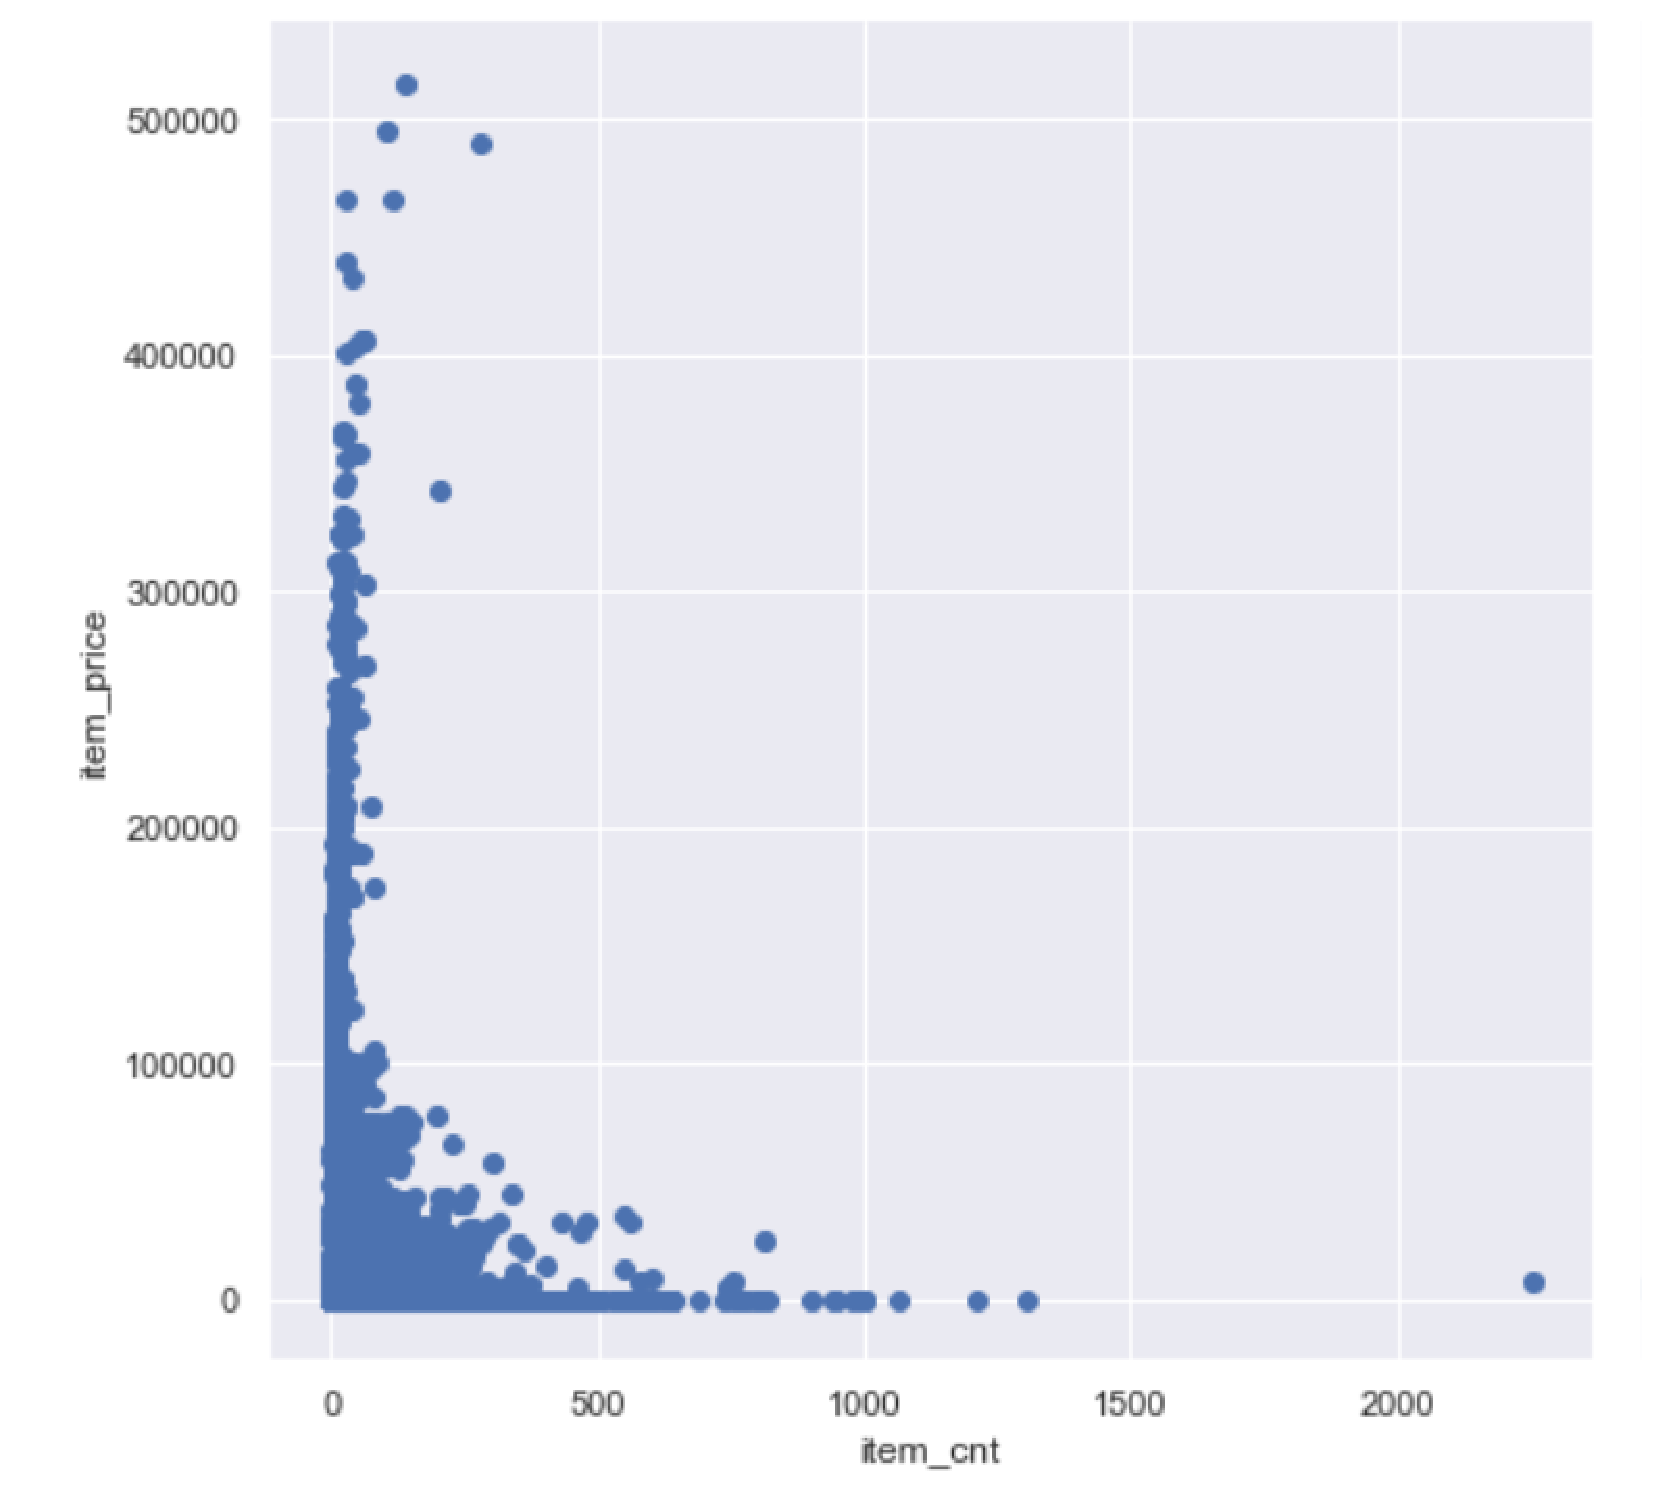
\includegraphics[width=0.5\textwidth,natwidth=780,natheight=703]{figures/outliers.eps}
      \caption{Checking for outliers}\label{Checking for outliers}
    \end{figure}
    
    %%==========================================================================================
    \begin{note}
    Last,
    we use the outlying degree to identify the specific group outlying aspects.
    
    The pseudo code of GOAM algorithm is as follows.
    The input is the group data,
    the output is outlying aspects of specific group ($G_1$).
    
    The details of the algorithm I will use an example to explain.
    \end{note}
%%==========================================================================================

\end{slide}
%%
%%==========================================================================================


%%==========================================================================================
%%

\section{Data Visualization}


%%==========================================================================================
\begin{slide}[toc=,bm=]{Extraction Time Features}

  \begin{itemize}
  \item
  We need to extract the time characteristics before drawing.
  
  \begin{itemize}
  \item
  Divide date_block_num into months and years.
 
  Get the title monthly_mean for item_cnt.mean.

  Get the title monthly_sum for item_cnt.sum.
 
  \end{itemize}
  \end{itemize}
  
  %%==========================================================================================
  \begin{note}
  The second challenge is how to evaluate the outlying degree of
  the query group between different aspects.
  
  In that case,
  we need to design a scoring function to measure the outlying degree.
  But adopting an appropriate scoring function without dimension bias still remains a problem.
  \end{note}
  %%==========================================================================================
  
  \end{slide}
%%
\begin{slide}{Annual Sales Performance}
  \begin{itemize}
    \item
    Look at the line chart below
    \begin{itemize}
      \item
      The average monthly sales are on the rise.
      
      \item
      Monthly sales reached their peak in December.
      \end{itemize}
    \end{itemize}
    
    \begin{figure}
      \centering
      \selectcolormodel{rgb}
      %\missingfigure{Testing.}
      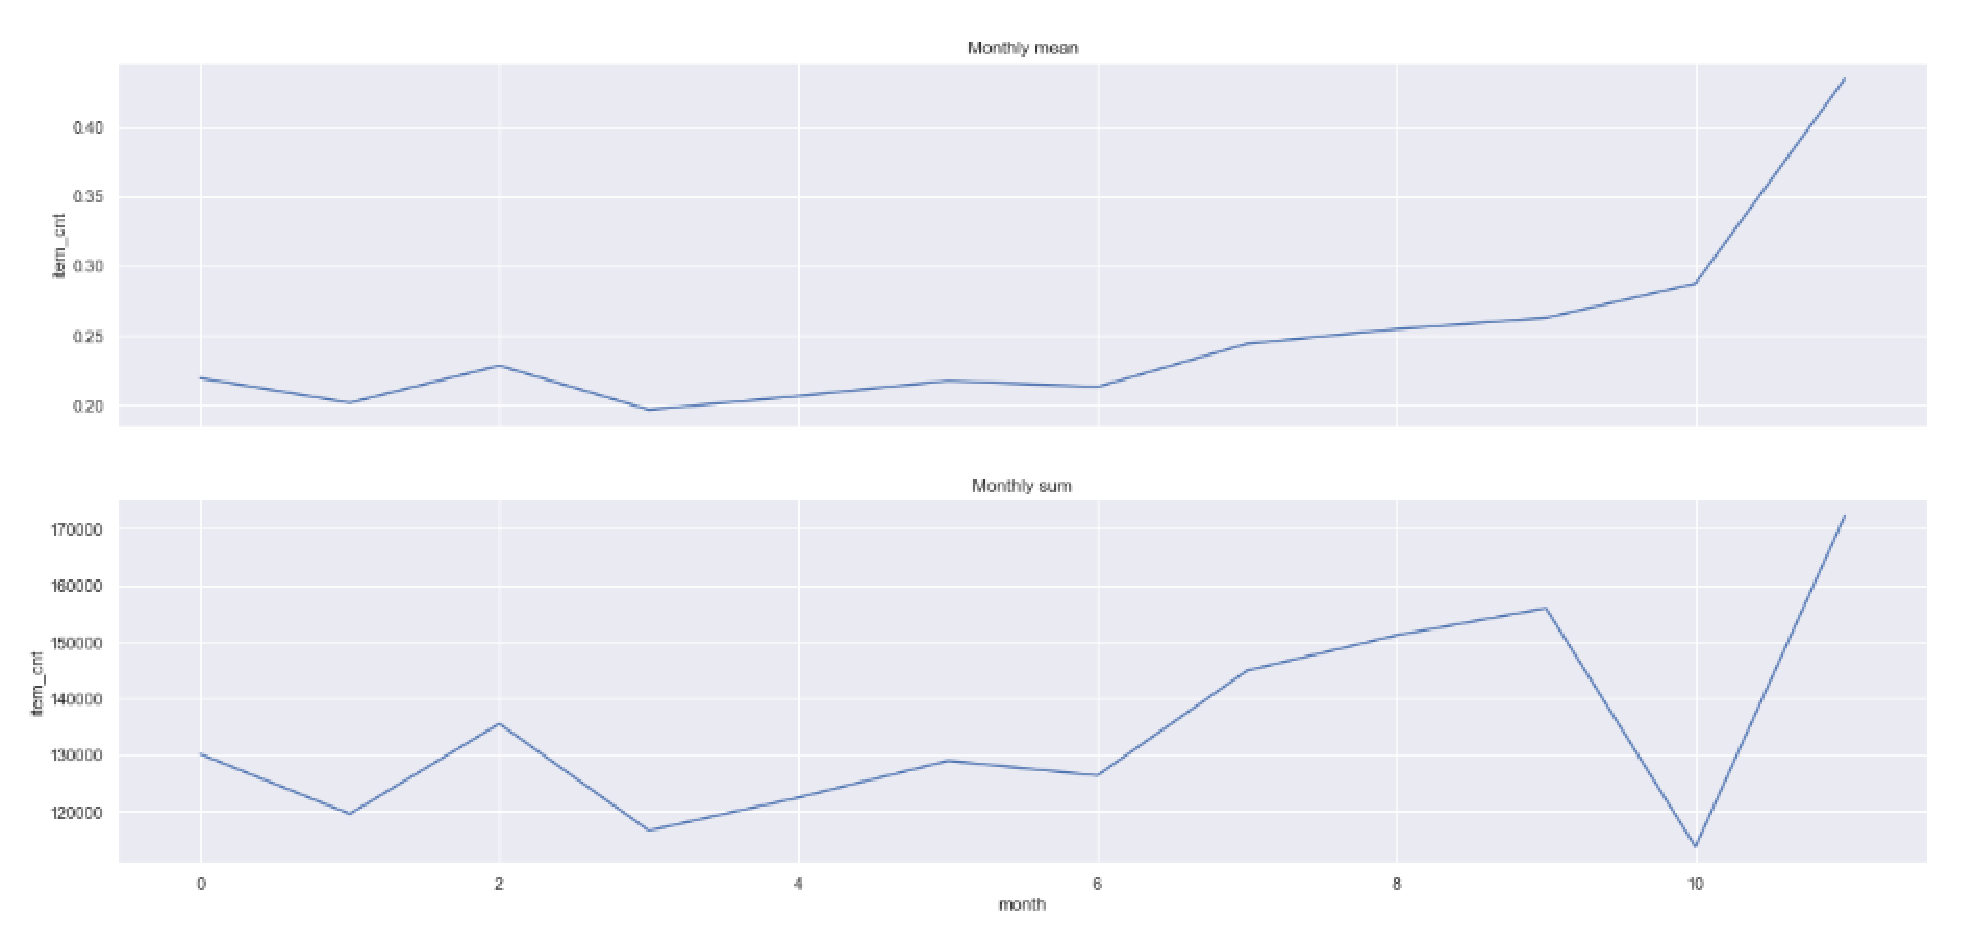
\includegraphics[width=0.7\textwidth,natwidth=938,natheight=436]{figures/line.eps}
      \caption{Annual sales performance}\label{Checking for outliers}
    \end{figure}
    
    %%==========================================================================================
    \begin{note}
    Last,
    we use the outlying degree to identify the specific group outlying aspects.
    
    The pseudo code of GOAM algorithm is as follows.
    The input is the group data,
    the output is outlying aspects of specific group ($G_1$).
    
    The details of the algorithm I will use an example to explain.
    \end{note}
%%==========================================================================================

\end{slide}
%%
%%==========================================================================================
\begin{slide}[toc=,bm=]{}
  \twocolumn
  {
    What category sells more?
  \begin{itemize}
  \item
  \smallskip
  Category 30 is the best seller.
  \item
  Also only few of the categories seems to hold most of the sell count.
 \end{itemize}
  \vspace{0.75cm}
  %\vspace{0.1cm}
  \begin{figure}
    \centering
    \selectcolormodel{rgb}
    %\missingfigure{Testing.}
    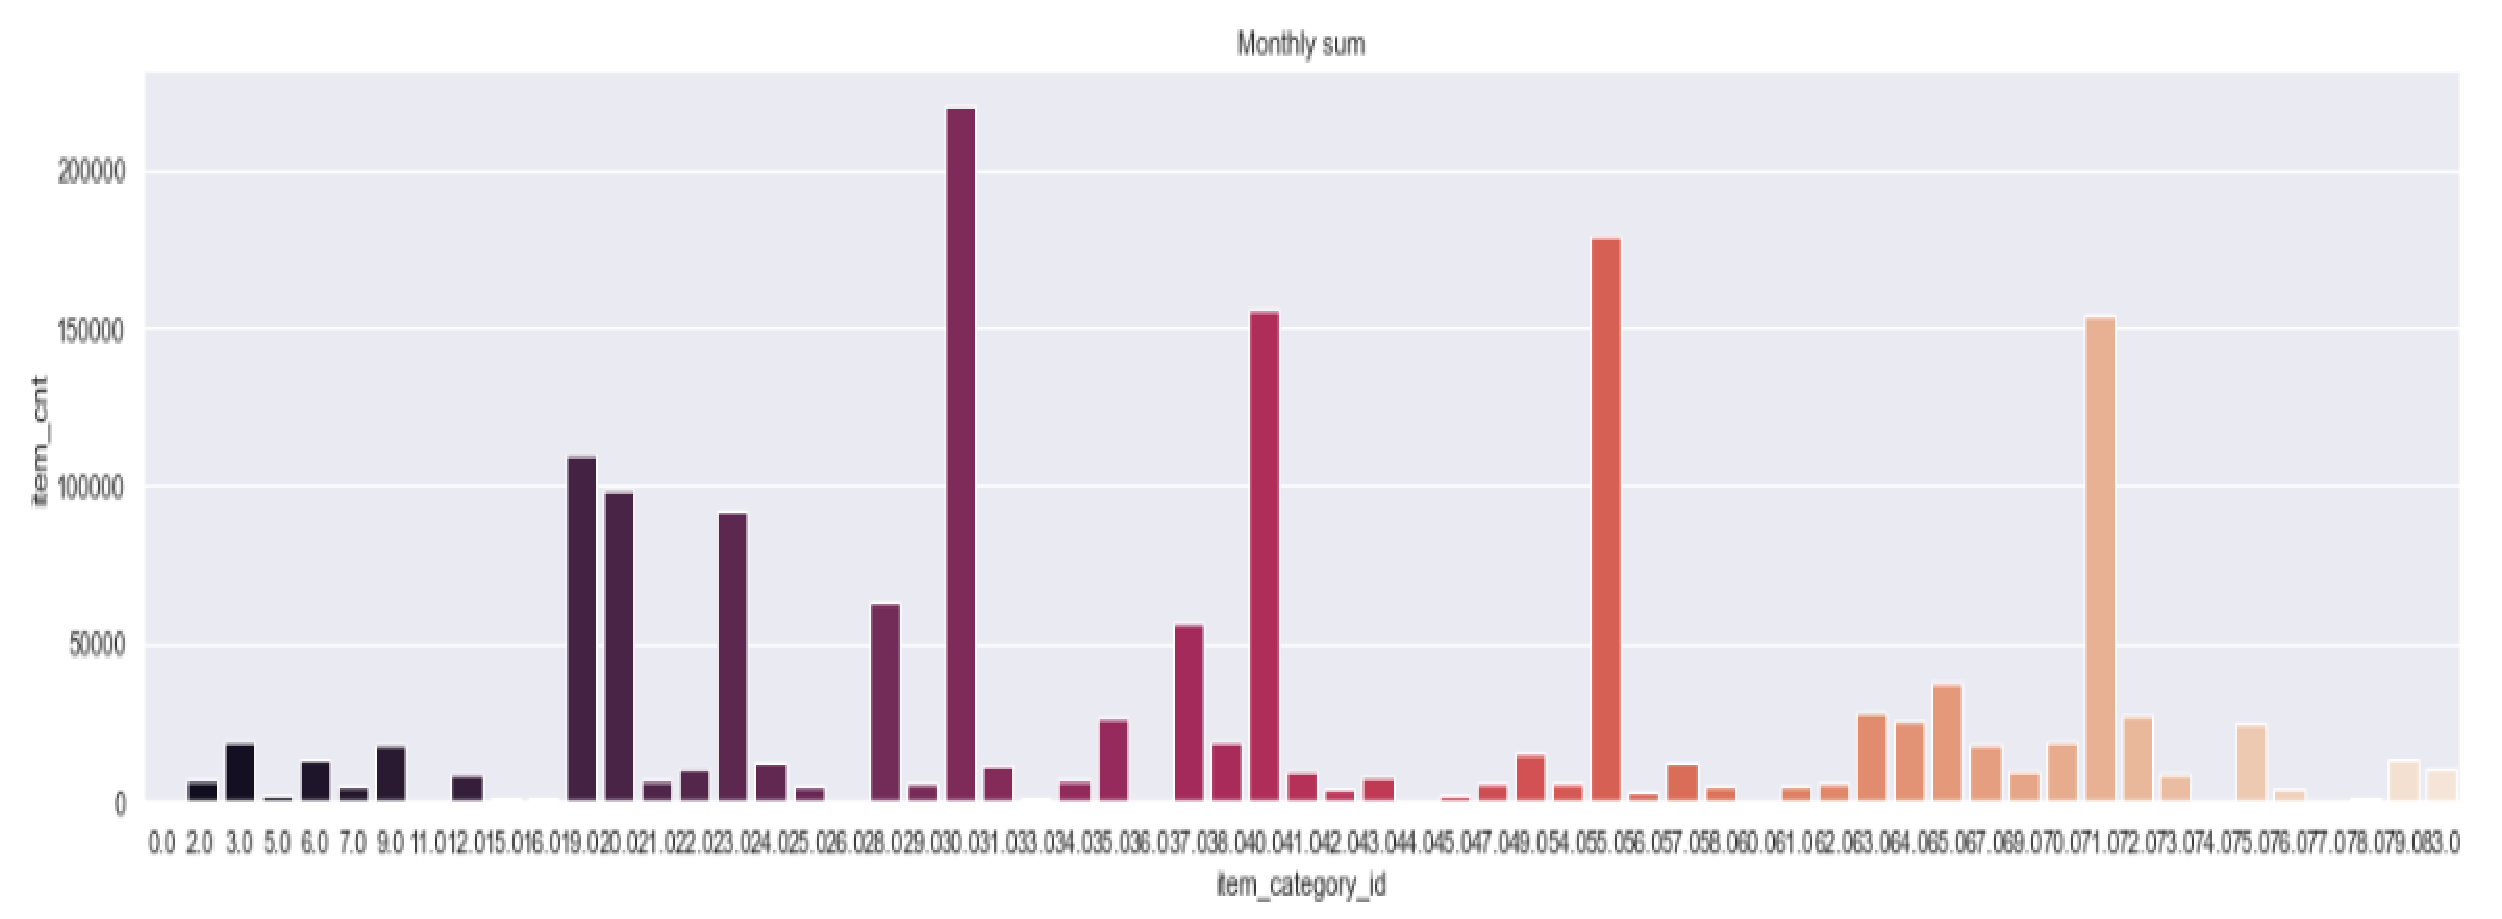
\includegraphics[width=1.0\textwidth,natwidth=1185,natheight=425]{figures/catg.eps}
    \caption{category}\label{Checking for outliers}
  \end{figure}
  }
  {
    What shop sells more?
  \begin{itemize}
  \item
  Most shops have similar sell rate.
  
  \item
   3 shops have a much higher rate, this is indicative of the shop size.
  \end{itemize}
  \bigskip
  \begin{figure}
    \centering
    \selectcolormodel{rgb}
    %\missingfigure{Testing.}
    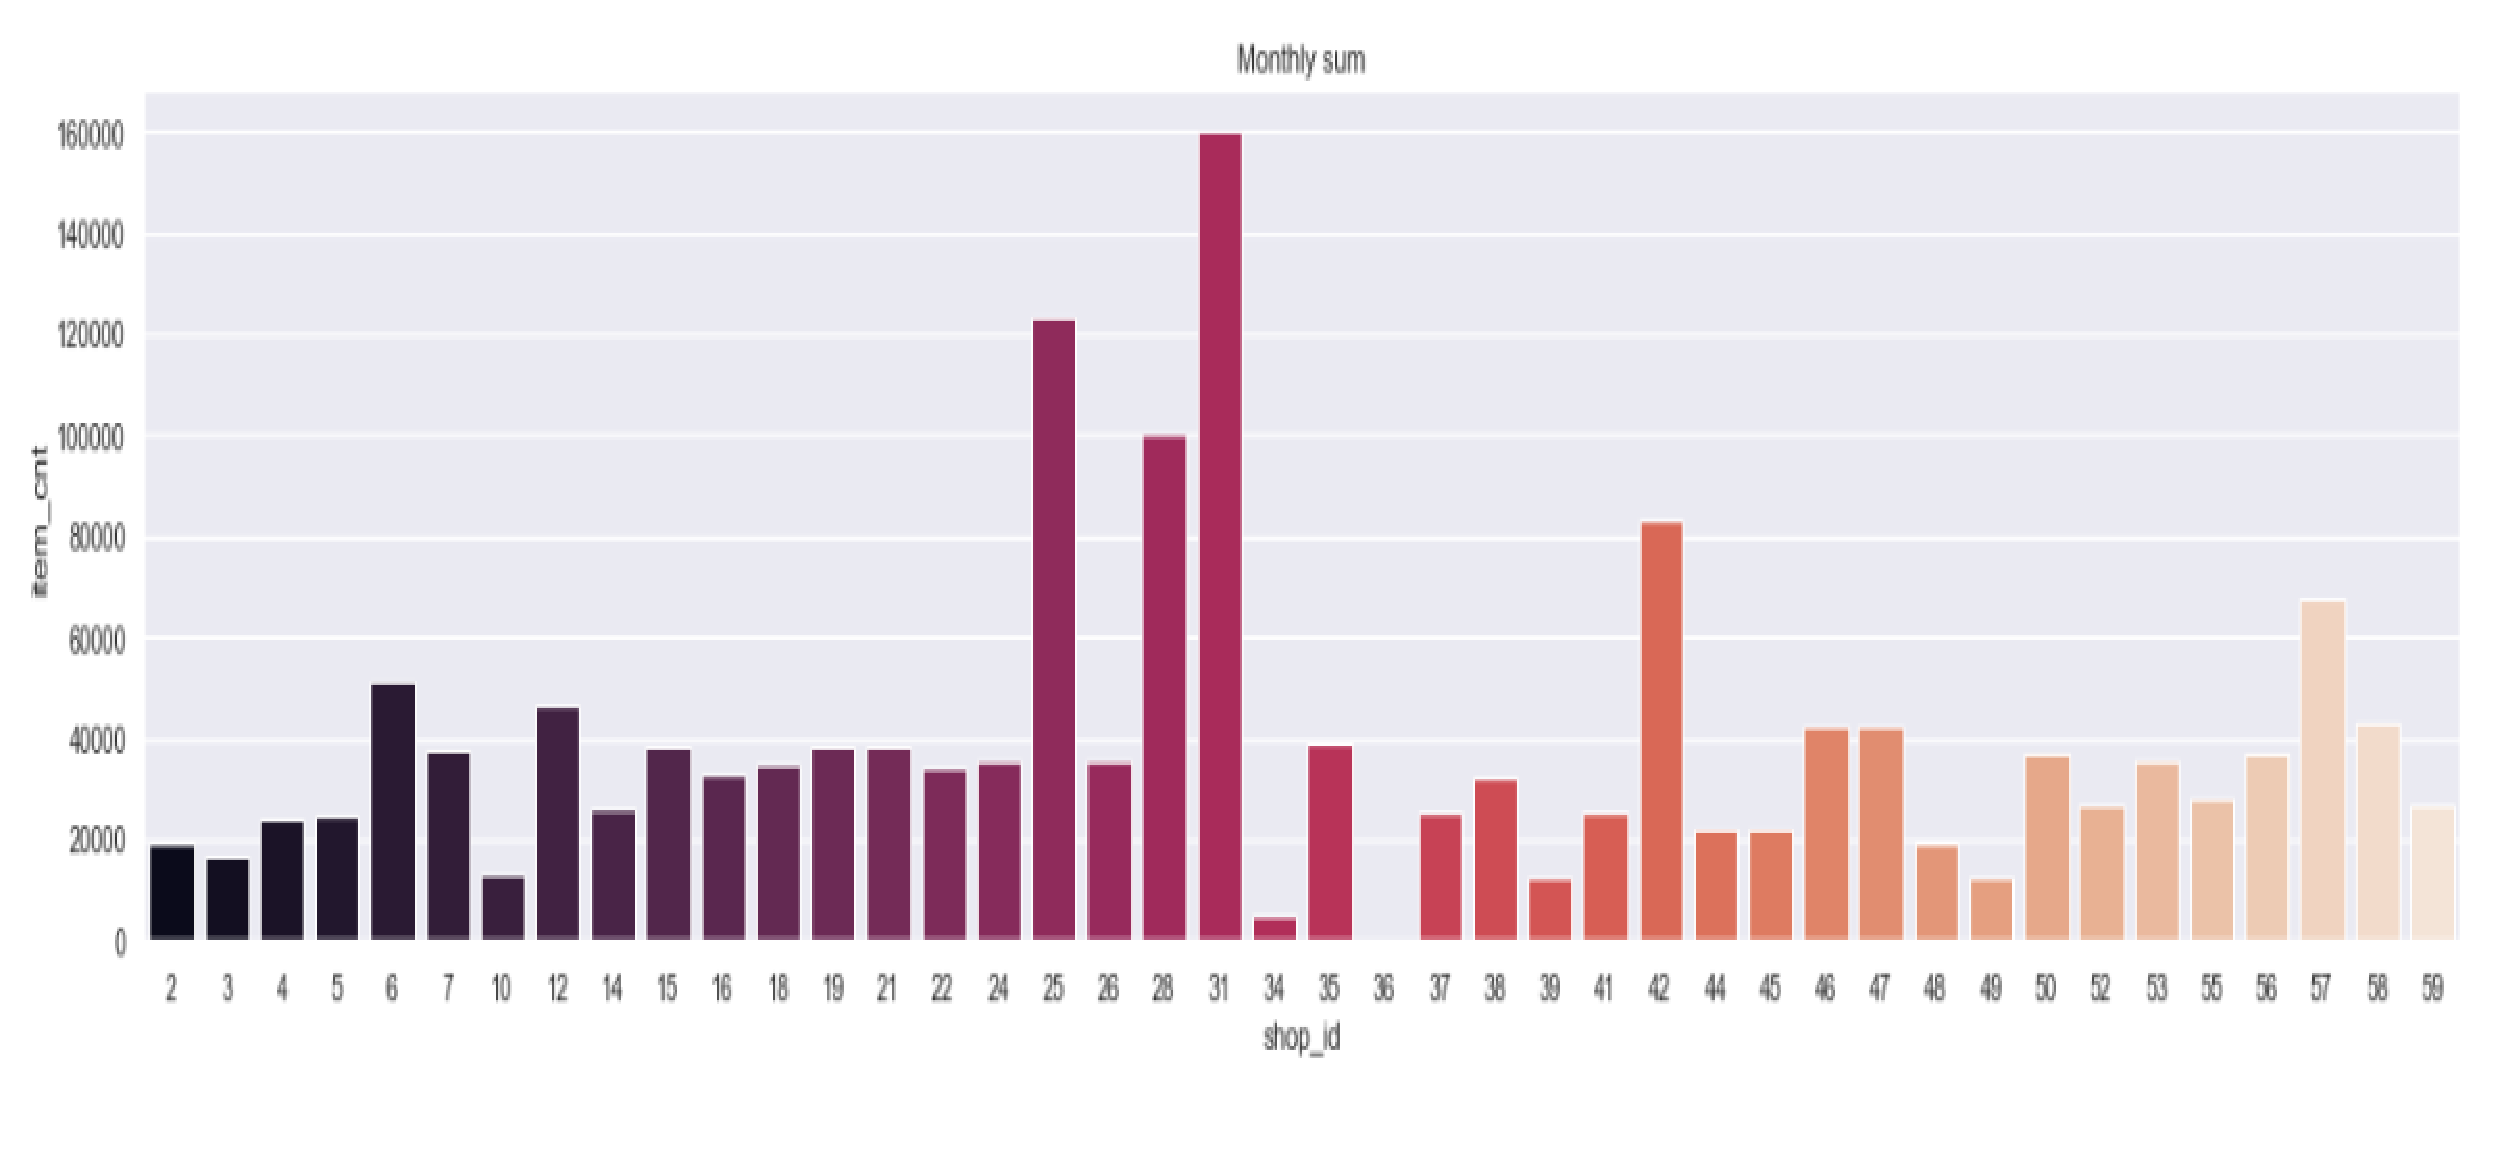
\includegraphics[width=1.0\textwidth,natwidth=1193,natheight=536]{figures/shop.eps}
    \caption{shop}\label{Checking for outliers}
  \end{figure}
  }
  
  %%==========================================================================================
  \begin{note}
  In this research paper,
  we proposed the group outlying aspects mining.
  Now,
  let me summarize the differences between group outlying aspects mining and outlying aspects mining.
  
  Group outlying aspects mining mainly focuses on the differences between groups.
  But outlying aspects mining mainly concentrates on the differences between objects.
  The target of group outlying aspects mining can be seen as many points.
  While the target of outlying aspects mining can be regarded as one point.
  
  In the NBA example,
  group outlying aspects mining focuses on the advantages
  or disadvantages of one team,
  however,
  outlying aspects mining focuses on the advantages or disadvantages of one player.
  \end{note}
  %%==========================================================================================
  
  \end{slide}
  \section{Feature Engineering}
  \begin{slide}[toc=,bm=]{Feature Extraction}

  \begin{itemize}
  \item
  We can extract new features from existing data.
  
  \begin{itemize}
  \item
  item_cnt_month:The monthly sales volume of each item in each store, sorted by month.
  \item
  hist_min(max)_item_price:Figure out the maximum and minimum monthly sales of each item by month.
  \item
  price_increace(decreace):How much each item's price changed from its (lowest/highest) historical price.
  \item
  item_cnt_max,item_cnt_mean,item_cnt_std:Maximum, minimum, average, and median monthly sales of each item in each store.
  \end{itemize}
  \end{itemize}
  
  %%==========================================================================================
  \begin{note}
  The second challenge is how to evaluate the outlying degree of
  the query group between different aspects.
  
  In that case,
  we need to design a scoring function to measure the outlying degree.
  But adopting an appropriate scoring function without dimension bias still remains a problem.
  \end{note}
  %%==========================================================================================
  
  \end{slide}
%%==========================================================================================
\begin{slide}[toc=,bm=]{Partition training set}
  \begin{itemize}
  \item
  \textcolor{orange}{Training set}
  
  \begin{itemize}
  \item
  Use the first three months to generate features and implement functionality.
  
  The 3-27 blocks are used for training.
  
  
  
  \end{itemize}
  
  \item
  \textcolor{orange}{Validation set}
  
  \begin{itemize}
  \item
  the five blocks 28-32 are used for verification.\\
  It is used to verify the accuracy of the model. The data is divided according to time because of its time characteristics.
  
  \end{itemize}
  \item
  \textcolor{orange}{Test set}
  
  \begin{itemize}
  \item
  We want to predict for "date_block_num" 34 so our test set will be block 33 and our predictions should reflect block 34 values.\\
  In other words we use block 33 because we want to forecast values for block 34.
  
  \end{itemize}
  \end{itemize}
  
  %%==========================================================================================
  \begin{note}
  In terms of the strengths of GOAM algorithm.
  
  I would like to talk about two main advantages of this algorithm.
  First is the reduction of complexity.
  GOAM algorithm utilizes the bottom up search method;
  what's more,
  it can reduce the size of candidate subspaces.
  
  Second is efficiency.
  The previous time complexity is O($2^d$);
  however,
  current time complexity if only O($d*n^2$).
  \end{note}
  %%==========================================================================================
  
  \end{slide}
%%
\begin{slide}{Mean Encoding}
  %Step Two - Outlying Degree Scoring
  \begin{itemize}
  \item
  Done after the train/validation split.
  
  \begin{itemize}
  \item
  Find the average monthly sales volume by store number.
  
  \item
  Find the average monthly sales volume by commodity number group.
  \item
  Find the average monthly sales volume of each item in each store, grouped by store and item number.
  \item
  Group by year, find the average annual sales.
  \item
  Group by month, find the average monthly sales.
  \end{itemize}
  \item
  Add meand encoding features to train set.
  Add meand encoding features to validation set.
  
  \end{itemize}
  
  %%==========================================================================================
  \begin{note}
  The second step is outlying degree scoring,
  which is to evaluate the outlying degree between the target group and competitive groups.
  
  First,
  we calculate the earth mover distance of one feature in different groups.
  
  The earth mover distance reflects the minimum mean distance between
  the target group and other groups on one feature.
  
  Later on,
  we utilize the EMD to measure the differences between groups.
  \end{note}
  %%==========================================================================================
  
  \end{slide}

%%
\section{Build Model}
\begin{slide}[toc=,bm=]{Linear Regression and Random Forest}
    %Step One - Group Feature Extraction}
    \begin{itemize}
      \item
      Linear Regression
      
      \begin{itemize}
      \item
      Train rmse: 0.7347132326333324\\
    Validation rmse: 0.7755311093532987
      
      
      
      \end{itemize}
      
      \item
      Random Forest
      
      \begin{itemize}
      \item
      Train rmse: 0.6985868322226099\\
  Validation rmse: 0.776123635046122
      
      \end{itemize}
      
      \end{itemize}
      
    
  
    
    %%==========================================================================================
    \begin{note}
    Now, let me specifically explain what each step means.
    The first step is group feature extraction.
    we can take one group extraction as an example.
    
    We suppose to use $f_1$, $f_2$, $f_3$ to represent three features of $G_q$.
    The values of $f_1$ are {$x_1$, $x_2$, $x_3$, $x_4$} and so on.
    And the values of $f_2$ are {$y_2$, $y_2$, $y_1$, $x_2$} and so on.
    
    For feature $f_1$,
    we use the histogram to illustrate feature $f_1$ after
    counting the frequency of each value,
    as show in figure 6 (a).
    
    Similarly,
    we can also extract other features of the group
    according to feature $f_1$.
    \end{note}
    %%==========================================================================================
    
    \end{slide}
%%
%%==========================================================================================
\begin{slide}[toc=,bm=]{XGBoost}
  %Step One - Group Feature Extraction}
  \begin{itemize}
  \item
  \smallskip
  Train rmse: 0.697475453300762\\
Validation rmse: 0.798117433161014
  \item
  XGBoost feature importance.
\end{itemize}
  
\begin{figure}
  \centering
  \selectcolormodel{rgb}
  %\missingfigure{Testing.}
  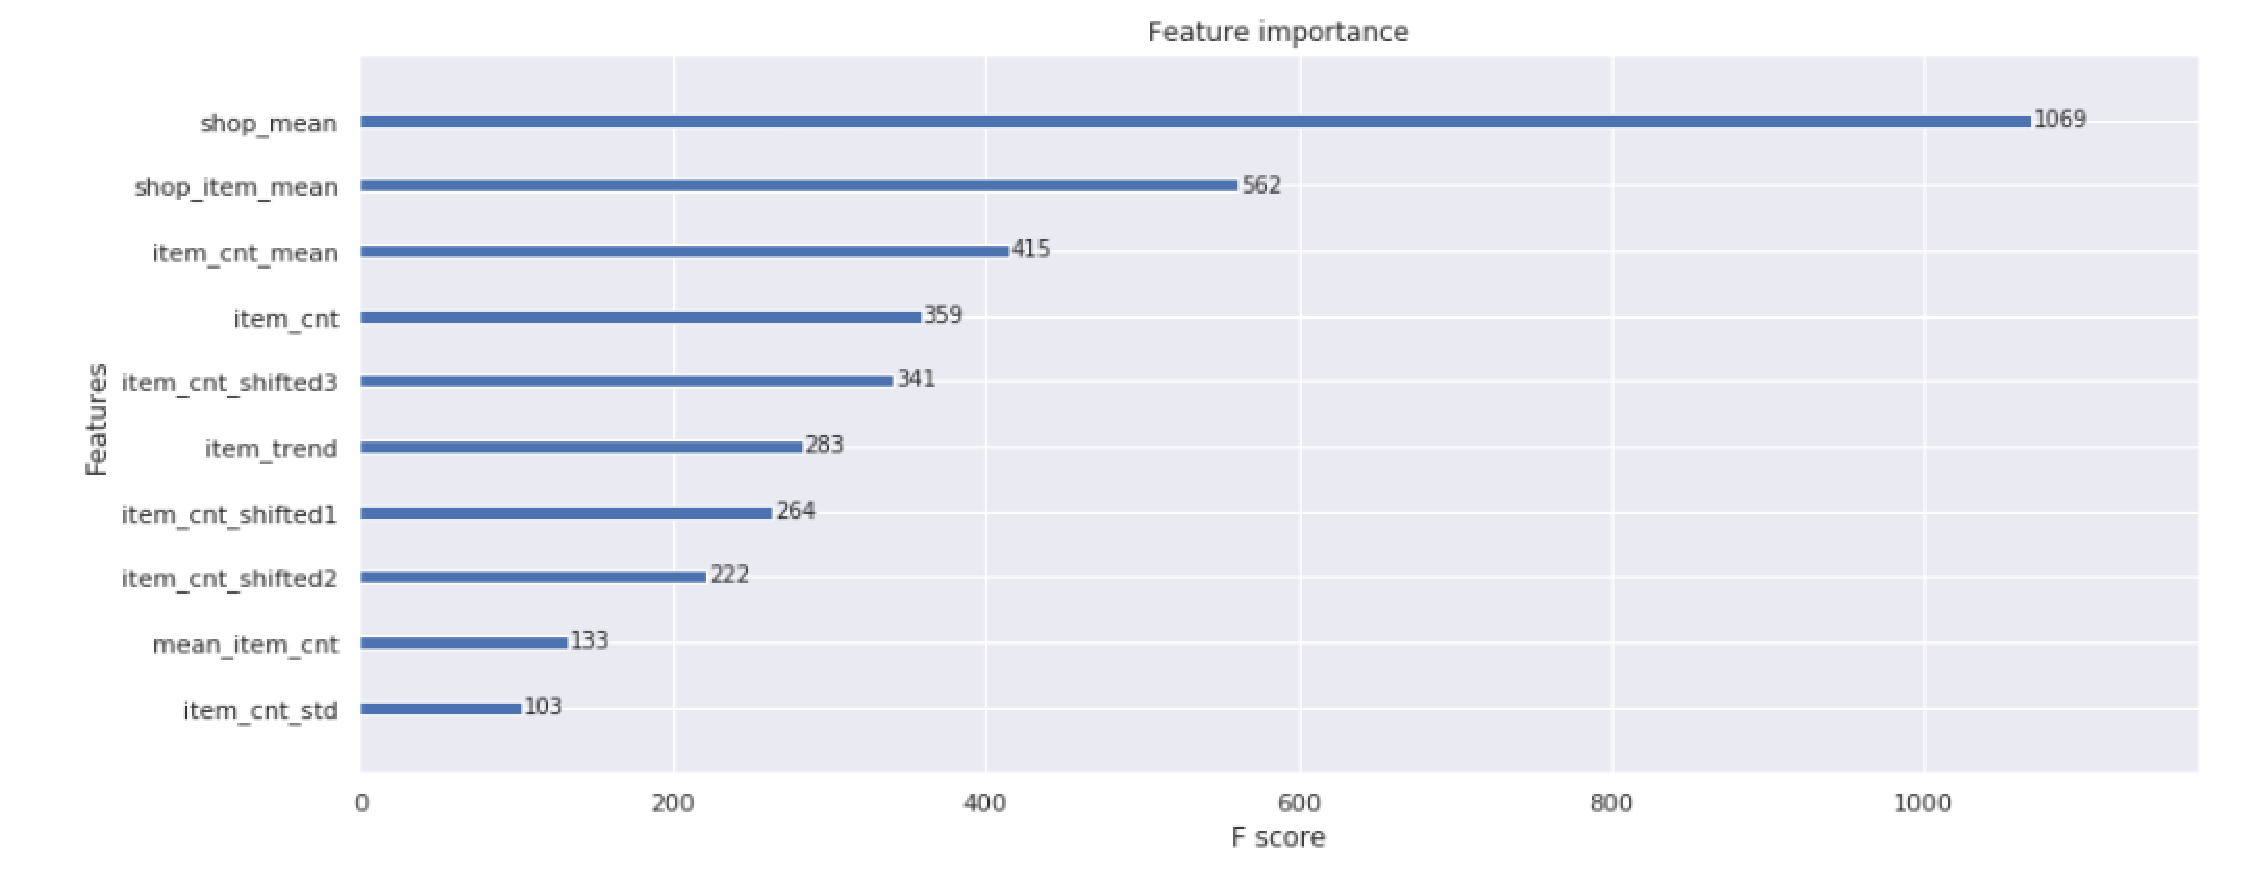
\includegraphics[width=0.7\textwidth,natwidth=1066,natheight=406]{figures/importance.eps}
  \caption{Feature importance}\label{Checking for outliers}
\end{figure}
  
  %%==========================================================================================
  \begin{note}
  Now, let me specifically explain what each step means.
  The first step is group feature extraction.
  we can take one group extraction as an example.
  
  We suppose to use $f_1$, $f_2$, $f_3$ to represent three features of $G_q$.
  The values of $f_1$ are {$x_1$, $x_2$, $x_3$, $x_4$} and so on.
  And the values of $f_2$ are {$y_2$, $y_2$, $y_1$, $x_2$} and so on.
  
  For feature $f_1$,
  we use the histogram to illustrate feature $f_1$ after
  counting the frequency of each value,
  as show in figure 6 (a).
  
  Similarly,
  we can also extract other features of the group
  according to feature $f_1$.
  \end{note}
  %%==========================================================================================
  
  \end{slide}
  \begin{slide}[toc=,bm=]{Create New Datasets}

    \begin{table}[tb]
    \setlength{\abovecaptionskip}{0pt}
    \setlength{\belowcaptionskip}{10pt}
    \centering
    \caption{Predictions from first level models}
    
    \begin{tabular}{ c | c | c | c }
    \toprule
      % after \\: \hline or \cline{col1-col2} \cline{col3-col4} ...
          &  random_forest    & linear_regression  & xgboost    \\
    \midrule
    0 &  0.98   &  0.85  &0.44   \\
    
    1 &  0.06   &  0.06 &0.10\\
    
    2 &   0.85   &  1.79 &0.50\\
    3 &   0.00   &  0.06 &0.10\\
    4 &   0.06   &  0.06 &0.10\\
    \bottomrule
    \end{tabular}
    \end{table}
    
    %%==========================================================================================
    \begin{note}
    From table $6$,
    we can see that GOAM method can identify the trivial outlying features
    and non-trivial outlying subspaces accurately and
    it is obvious from the table that the accuracy of GOAM is the best,
    which is 100\%.
    
    This is because the outlying aspects mining method
    can't obtain the features of a group and the scoring function
    is based on point to point metric.
    Therefore,
    it is not suitable for group outlying aspects mining.
    \end{note}
    %%==========================================================================================
    
    \end{slide}
    %%
    %%==========================================================================================
\begin{slide}[toc=,bm=]{Ensembling}

\begin{center}
\begin{itemize}

\item
\smallskip
\large
{To combine the 1st level model predictions,to use a simple linear regression. \\
This is the model that will combine the other ones to hopefully make an overall better prediction. \\

\item
Make predictions on test set using the 1st level models predictions as features.
}

\end{itemize}
\end{center}
\end{slide}
\begin{slide}{Ensemble Diagram}
  \begin{itemize}
    \item
    Look at the line chart below
    \begin{itemize}
      \item
      Here is an image to help the understanding
      
      
      \end{itemize}
    \end{itemize}
    
    \begin{figure}
      \centering
      \selectcolormodel{rgb}
      %\missingfigure{Testing.}
      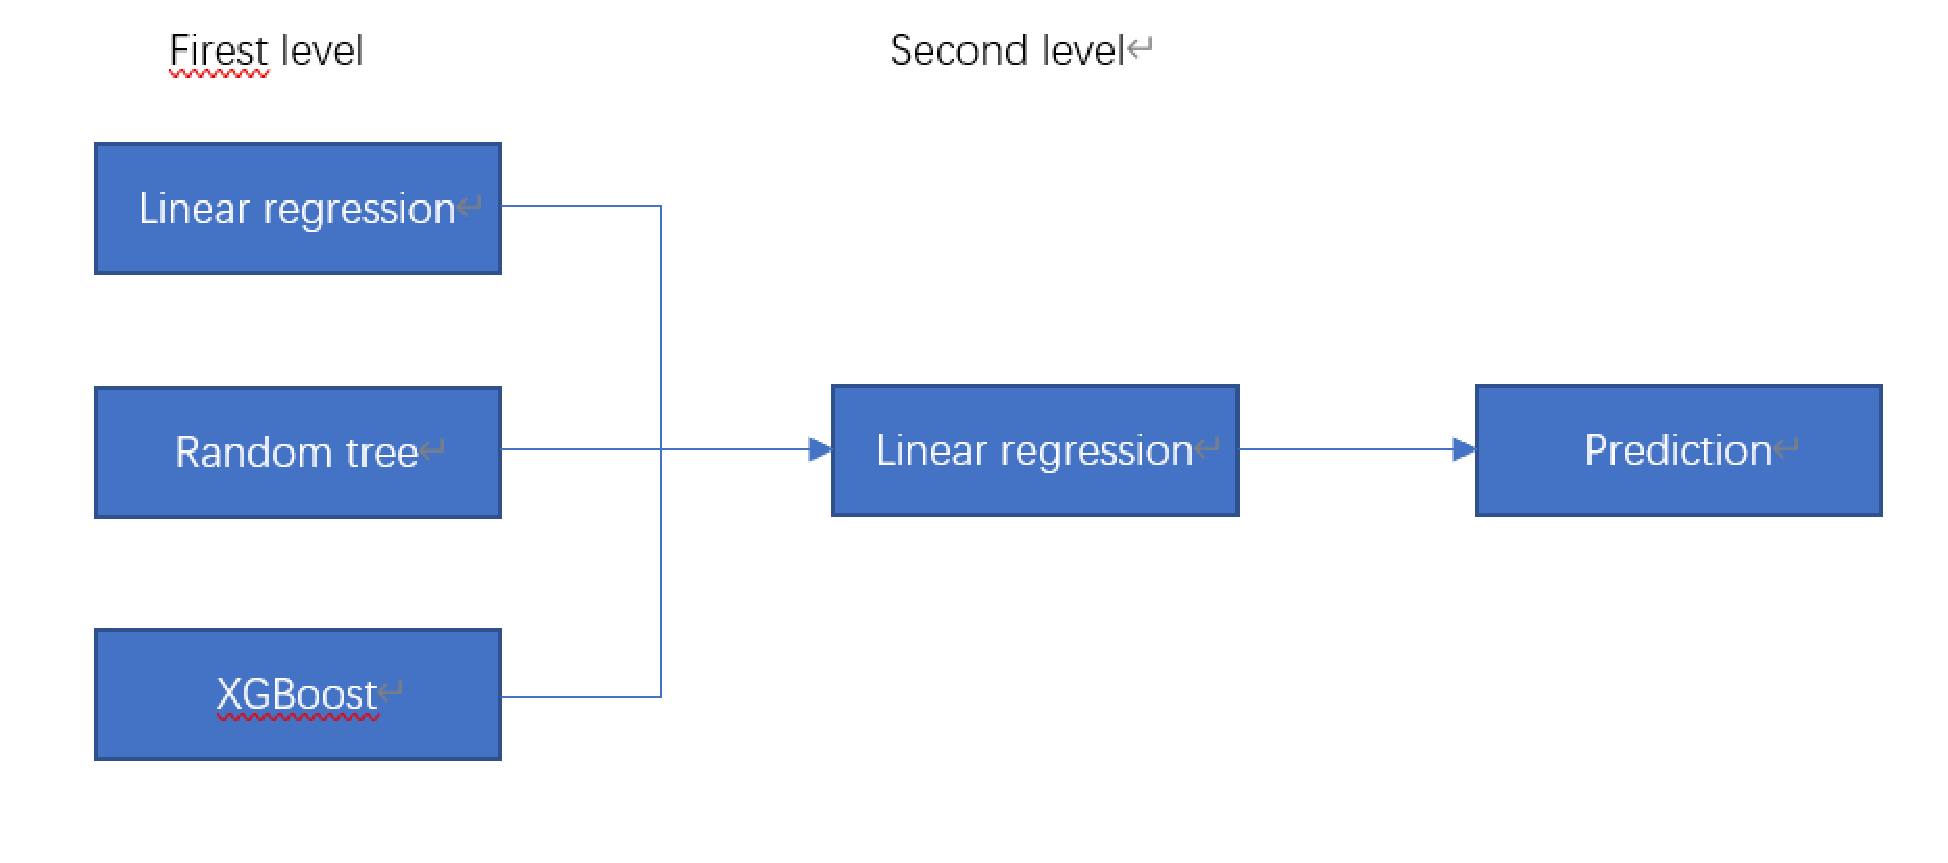
\includegraphics[width=0.7\textwidth,natwidth=919,natheight=398]{figures/ensemble.eps}
      \caption{Ensemble diagram}\label{Checking for outliers}
    \end{figure}
    
    %%==========================================================================================
    \begin{note}
    Last,
    we use the outlying degree to identify the specific group outlying aspects.
    
    The pseudo code of GOAM algorithm is as follows.
    The input is the group data,
    the output is outlying aspects of specific group ($G_1$).
    
    The details of the algorithm I will use an example to explain.
    \end{note}
%%==========================================================================================

\end{slide}
\begin{slide}[toc=,bm=]{Output Dataframe}

  \begin{table}[tb]
  \setlength{\abovecaptionskip}{0pt}
  \setlength{\belowcaptionskip}{10pt}
  \centering
  \caption{Output dataframe}
  
  \begin{tabular}{ c | c | c }
  \toprule
    % after \\: \hline or \cline{col1-col2} \cline{col3-col4} ...
    &  ID    & item_cnt_month      \\
    \midrule
    0 &  0  &  0.85     \\
    
    1 &  1   &  0.08 \\
    
    2 &   2   &  1.29 \\
    3 &   3  &  0.06 \\
    4 &   4   &  0.08 \\
    5 &  5   &  0.96 \\
    6 &  6  &  1.25 \\
    7 &  7   &  0.21 \\
    8 &  8   &  1.99 \\
    9 &  9   &  0.06 \\
  \bottomrule
  \end{tabular}
  \end{table}
  
  %%==========================================================================================
  \begin{note}
  From table $6$,
  we can see that GOAM method can identify the trivial outlying features
  and non-trivial outlying subspaces accurately and
  it is obvious from the table that the accuracy of GOAM is the best,
  which is 100\%.
  
  This is because the outlying aspects mining method
  can't obtain the features of a group and the scoring function
  is based on point to point metric.
  Therefore,
  it is not suitable for group outlying aspects mining.
  \end{note}
  %%==========================================================================================
  
  \end{slide}   

%%==========================================================================================
%%


%%==========================================================================================
% TODO: Contact Page
\begin{wideslide}[toc=,bm=]{Contact Information}
\centering
\vspace{\stretch{1}}
\twocolumn[
lcolwidth=0.35\linewidth,
rcolwidth=0.65\linewidth
]
{
% \centerline{
\includegraphics[scale=.2]{tulip-logo.eps}}
}
{
\vspace{\stretch{1}}
Thank you for listening!\\
Siyu Chen\\
Xi'an Shiyou University\\
\begin{description}
 \item[\textcolor{orange}{\faEnvelope}] \href{mailto:785987165@qq.com}
 {\textsc{\footnotesize{785987165@qq.com}}}

 
\end{description}
}
\vspace{\stretch{1}}
\end{wideslide}

\end{document}

\endinput
